%META {"question":"Nhận xét nào ĐÚNG về hai tia Ox và Oy trong hình?","options":["Ox và Oy là hai tia đối nhau vì chung gốc O và hợp thành một đường thẳng","Ox và Oy không là hai tia đối nhau vì chúng tạo thành góc nhỏ hơn 180°","Ox và Oy trùng nhau","Không thể xác định"],"answer":0,"note":"Hai tia đối nhau: chung gốc O và cùng nằm trên một đường thẳng — ở đây góc xOy bằng 180°."}
\documentclass[border=5pt]{standalone}
\usepackage{tkz-euclide}
\usetikzlibrary{arrows.meta}
% Màu dùng chung cho toàn bộ hình vẽ (ảnh stack với nền tối của web)
\definecolor{tminc}{RGB}{226,232,240}   % chữ + nét chính
\definecolor{tmblue}{RGB}{0,210,255}    % nhấn neon xanh
\definecolor{tmpink}{RGB}{255,0,200}    % nhấn neon hồng
\definecolor{tmgreen}{RGB}{0,255,136}   % nhấn neon xanh lá
\color{tminc}

\begin{document}
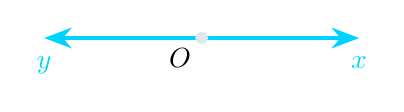
\begin{tikzpicture}[line width=1.1pt,>={Stealth[length=3.5mm]}]
  \coordinate (O) at (0,0);
  \coordinate (X) at (2,0);
  \coordinate (Y) at (-2,0);
  \draw[tmblue,->] (O) -- (X) node[below=3pt]{$x$};
  \draw[tmblue,->] (O) -- (Y) node[below=3pt]{$y$};
  \tkzDrawPoints[size=3.5,color=tminc,fill=tminc](O)
  \tkzLabelPoint[below left](O){$O$}
\end{tikzpicture}
\end{document}
